\documentclass[a4paper,11pt,fleqn]{scrartcl}%fleqn pour aligner les equations à gauche

\usepackage{../../Styles/Cours}

\newcommand{\chnum}{Chapitre 06}
\newcommand{\chtitle}{Réalisation d'une pile}
\newcommand{\dtype}{TP}

  
\begin{document}
\maketitle

\textbf{Objectifs : } De nombreux objets du quotidien utilisent de l'énergie électrique. une pile électrochimique est une source d'énergie autonome. \textbf{Quel est le principe de fonctionnement d'une pile ?}\\

\noindent\begin{minipage}{.98\textwidth}
\begin{documentboxenv}{Protocole expérimental 1}
\begin{itemize*}
	\item Dans un bécher, mélanger deux solutions de sulfate de cuivre et de sulfate de zinc de même volume et de même concentration en quantité de matière $c$ = \SI{0.1}{\mole\per\liter}.
	\item Plonger une lame de cuivre et une lame de zinc dans la solution obtenue.
\end{itemize*}
\end{documentboxenv}
\end{minipage}


\noindent\begin{minipage}[t][12.5cm][t]{.49\linewidth}
\begin{documentboxenv}{Capacité d'une pile}
La capacité électrique d'une pile, notée $Q_{max}$, est la charge électrique maximale (en coulomb \unit{\coulomb}) que la pile peut débiter durant toute sa durée de vie.\\
	$$Q_{max}=n_{\ce{e-},ech,max} \times N_A \times e$$
	 $Q_{max}$ : charge de la pile en coulomb (\unit{\coulomb})\\
	 $n_{\ce{e-},ech,max}$ : quantité maximale d'électrons échangés en mole (\unit{\mole})\\
	$N_A$ : constante d'Avogadro ($N_A \approx$ \num{6,02e23} \unit{\per \mole})\\
	$e$ : charge élémentaire ($e \approx$ \num{1,60e-19} \unit{\coulomb})\\
\end{documentboxenv}	
\begin{documentboxenv}{Données}
\begin{itemize}
	\item Les ions cuivre (II) \ce{Cu^2+(aq)} donnent une coloration bleue à la solution qui les contient.
	\item Couples oxydant/réducteur : \ce{Cu^2+}/\ce{Cu} et \ce{Zn^2+}/\ce{Zn}
\end{itemize}
\end{documentboxenv}
\end{minipage}
\begin{minipage}[t][12.5cm][t]{.49\linewidth}
\begin{documentboxenv}{Protocole expérimental 2}
\begin{center}
	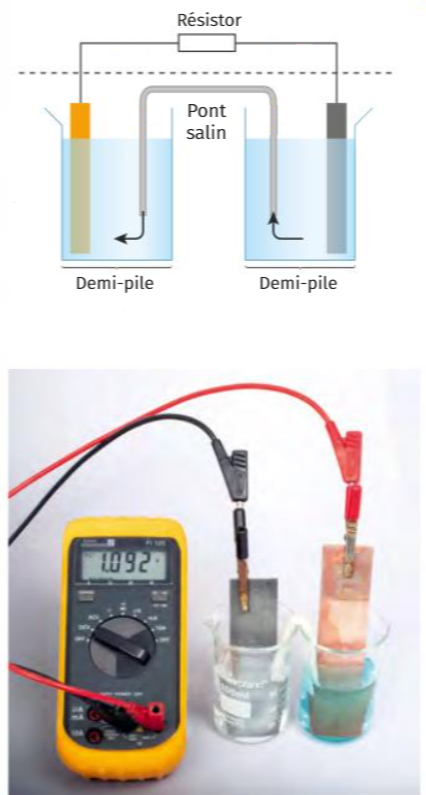
\includegraphics[width = .8\linewidth]{Ressources/TSPE_C7_AE2_Fig1.png}
\end{center}
\end{documentboxenv}
\end{minipage}

\section*{Protocole expérimental 1}
\begin{enumerate}
	\item Observer l'expérience réalisée. En déduire l'équation de la réaction modélisant la transformation chimique.
	\item Justifier l'expression "\emph{transfert spontané d'électrons par contact direct entre réactifs}".

	\item La constante d'équilibre de l'équation est \num{1E37}. Montrer que le sens d'évolution spontanée prévu est compatible avec les observations expérimentales.
\end{enumerate}
\newpage
\section*{Protocole expérimental 2}
\begin{enumerate}[resume]
	\item Noter le sens conventionnel du courant.
	\item Quel est l'intérêt d'ajouter un résistor au montage ?
	\item Retirer le pont salin. Noter les observations. Formuler une hypothèse sur le rôle du pont salin.
	\item A l'aide du sens du courant observé, déterminer si la réaction ayant lieu à chaque électrode est une oxydation ou une réduction.
	\item Écrire l'équation de la réaction associée à la transformation ayant lieu lors du fonctionnement de la pile.
	\item Compléter le schéma de la pile fourni.
	\item Justifier l'expression "\emph{transfert spontané d'électrons par l'intermédiaire d'un circuit extérieur}".
	\item Déterminer la tension à vide de la pile, c'est à dire la tension mesurée entre ses électrodes quand le circuit est ouvert.
	\item Dans le cas où il y a \SI{1.00E-2}{\mole} de zinc consommé, déterminer la capacité de la pile.
\end{enumerate}

\vspace{3cm}
\begin{figure}[h!]
    \centering
    \caption*{\textbf{Schéma de la pile}}
    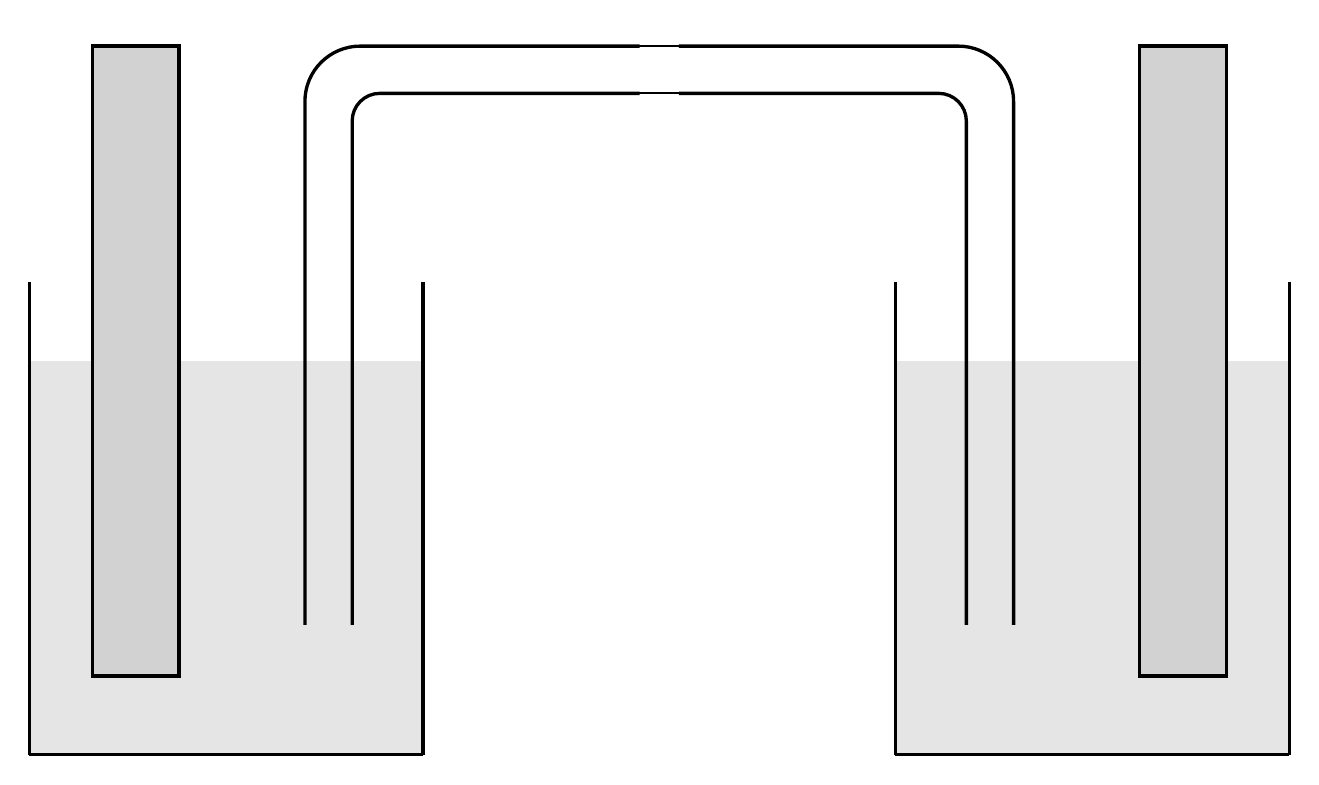
\begin{tikzpicture}[scale=2,transform shape]
    %%%%%%%%%%%%%%%%%%%%%%%%%%%%%%%%%%%%%% Béchers
    \fill[gray!20] (-1.5,0)--(-4,0)--(-4,2.5)--(-1.5,2.5)--cycle;
    \fill[gray!20] (1.5,0)--(4,0)--(4,2.5)--(1.5,2.5)--cycle;
    
    \draw[very thick] (-1.5,0)--(-1.5,3);
    \draw[very thick] (-1.5,0)--(-4,0);
    \draw[very thick] (-4,0)--(-4,3);

    \draw[very thick] (1.5,0)--(1.5,3);
    \draw[very thick] (1.5,0)--(4,0);
    \draw[very thick] (4,0)--(4,3);

    %%%%%%%%%%%%%%%%%%%%%%%%%%%%%%%%%%%%%% Plaques
    \filldraw[gray!35,draw=black, very thick] (-3.05,0.5)--(-3.6,0.5)--(-3.6,4.5)--(-3.05,4.5)--cycle;
    \filldraw[gray!35,draw=black, very thick] (3.05,0.5)--(3.6,0.5)--(3.6,4.5)--(3.05,4.5)--cycle;

    %%%%%%%%%%%%%%%%%%%%%%%%%%%%%%%%%%%%%% Pont salin
    \tikzstyle{suite}=[-,very thick,rounded corners=10pt]
    \node (b1) at (1.95,0.7){};
    \node (a1) at (-1.95,0.7){};
    \node (i1) at (0,4.2){};

    \draw[suite] (b1)|-(i1)-|(a1.north) ;
    
    \node (b2) at (2.25,0.7){};
    \node (a2) at (-2.25,0.7){};
    \node (i2) at (0,4.5){};
    \tikzstyle{suite2}=[-,very thick,rounded corners=20pt]
    \draw[suite2] (b2)|-(i2)-|(a2.north) ;
    \draw[thick] (-0.2,4.2) -- (0.2,4.2);
    \draw[thick] (-0.2,4.5) -- (0.2,4.5);
\end{tikzpicture}
\end{figure}
\end{document}